%%*************************************************************************
%% Legal Notice:
%% This code is offered as-is without any warranty either expressed or
%% implied; without even the implied warranty of MERCHANTABILITY or
%% FITNESS FOR A PARTICULAR PURPOSE! 
%% User assumes all risk.
%% In no event shall IEEE or any contributor to this code be liable for
%% any damages or losses, including, but not limited to, incidental,
%% consequential, or any other damages, resulting from the use or misuse
%% of any information contained here.
%%
%% All comments are the opinions of their respective authors and are not
%% necessarily endorsed by the IEEE.
%%
%% This work is distributed under the LaTeX Project Public License (LPPL)
%% ( http://www.latex-project.org/ ) version 1.3, and may be freely used,
%% distributed and modified. A copy of the LPPL, version 1.3, is included
%% in the base LaTeX documentation of all distributions of LaTeX released
%% 2003/12/01 or later.
%% Retain all contribution notices and credits.
%% ** Modified files should be clearly indicated as such, including  **
%% ** renaming them and changing author support contact information. **
%%
%% File list of work: IEEEtran.cls, IEEEtran_HOWTO.pdf, bare_adv.tex,
%%                    bare_conf.tex, bare_jrnl.tex, bare_jrnl_compsoc.tex
%%*************************************************************************

\documentclass[10pt, conference, compsocconf]{IEEEtran}

\usepackage{ucs}
\usepackage[utf8x]{inputenc}
\usepackage[english]{babel}
\usepackage{hyperref}     % use \url{http://$URL} or \href{http://$URL}{Name}
\usepackage{underscore}   % underscores need not be escaped
\usepackage{subfigure}
\usepackage{verbatim}
\usepackage{moreverb}
\usepackage{float}
\usepackage{booktabs}     % professional tables
\usepackage{listings}
\usepackage{color}
\usepackage{amsmath}
\usepackage{indentfirst}
\usepackage{epstopdf}
\definecolor{darkgreen}{rgb}{0,0.4,0}
\lstset{language=C,captionpos=b,tabsize=3,frame=lines,keywordstyle=\color{blue},commentstyle=\color{darkgreen},stringstyle=\color{red},numbers=left,numberstyle=\tiny,numbersep=5pt,breaklines=true,showstringspaces=false,basicstyle=\footnotesize,emph={label}}

% Support for including graphics
\usepackage{graphicx}
\DeclareGraphicsExtensions{.pdf,.png,.jpg}

\begin{document}

\title{SourceDotCode online compiler}

\author{\IEEEauthorblockN{Tudor Cornea}
\IEEEauthorblockA{Computer Science and Engineering Department\\
University POLITEHNICA of Bucharest\\
Bucharest, Romania\\
\emph{tudor.cornea@gmail.com}}
}

% make the title area
\maketitle


\begin{abstract}
  % vim: set tw=78 sts=2 sw=2 ts=8 aw et ai:

There are times when we have a certain program to compile, but we lack the tools to do so. An example would be if we are using a low-powered device, like a mobile phone, or a Tablet. SourceDotCode allows us to test simple programs, see if they compile successfully, and inspect the output. In the following sections, I will talk about the main challenges I had when writing SourceDotCode, and how I managed to overcome them.



\end{abstract}

\begin{IEEEkeywords}
Compilation; Web Service; ptrace;
\end{IEEEkeywords}

% For peerreview papers, this IEEEtran command inserts a page break and
% creates the second title. It will be ignored for other modes.
\IEEEpeerreviewmaketitle

\section{Introduction}
\label{sec:intro}
% vim: set tw=78 sts=2 sw=2 ts=8 aw et ai:

We define Compile as a Service (CAAS), as a function taking as input a superset of the following parameters:
\begin{enumerate}
\item{Source code}
\item{Language}
\item{Architecture}
\end{enumerate}
and providing as output the execution result of running the program.


As an inspiration for this project I had two platforms: 
\begin{enumerate}
\item{Infoarena}
\item{VMChecker}
\end{enumerate}

They are both great platforms, but they are rigid, in the sense that they are targeted to certain operations.
They are not general purpose compilation platforms, which forms the scope of my project.

Infoarena only allows submitting code for certain programming challenges.
As supported languages, it only allows submitting C and C++ code, differentiating between them by the file extension.

VMChecker, is the platform for evaluating homeworks for a good amount of subjects, inside the Faculty of Automatic Control and Computers.
It is a bit more complex than Infoarena, and it allows compiling programs in a greater amount of programming languages.
Programs are typically compiled and run inside a Virtual Machine environment, hence the name "VMChecker".


When designing an online compilation tool, there are certain challenges, most notably:
\begin{enumerate}
\item{Scalability}
\item{Security}
\end{enumerate}

Scalability refers to how the application is going to handle a large number of incoming requests.
Common bottlenecks in such applications occur between the Web Server and Database, and between the Web Server and secodary resources (Ex: When calling another Web Service for a specific task).

The security issues that may arise in our case deal with the code execution.
Allowing the user to execute arbitrary code on your machine would pose a huge risk.
For example, he could attempt to reboot the machine, or create sockets and flood a destination with ICMP packets.

In the next section, we are going to explore a way to overcome this problem.










 


\section{Architectural Model}
\label{sec:model}
% vim: set tw=78 sts=2 sw=2 ts=8 aw et ai:

The solution I used for SourceDotCode involves a Supervisor process, which will monitor the execution of a program, and terminate its execution when encountering certain "dangerous" system calls.

Examples of such system calls are:
\begin{enumerate}
\item{sys_reboot}
\item{sys_socketcall}
\item{sys_clone}
\item{sys_unlink}
\end{enumerate}

The Linux Kernel provides ptrace, a consistent interface to implement this feature, which is commonly used by debugging software like gdb, or strace.
The supervisor process will make use of the ptrace system call to monitor the execution of the main program, as we can see in [fig1].

\begin{figure}
\begin{center}
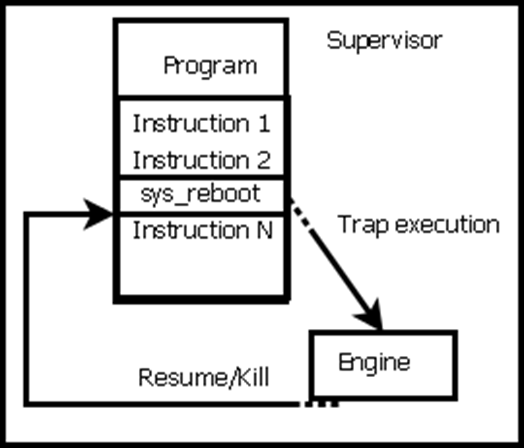
\includegraphics[scale=0.5]{pics/superv.png}
\caption{Supervisor model}
\end{center}
\label{fig1:superv}
\end{figure}

The complete architecture of the service is shown in [fig2].
There will be a Web Service Client, which sends requests to the Web Server in the form of JSON messages.
The Web Server will receive the requests, and dispatch them to a Build Agent entity.

The Build Agent will be responsible with providing the runtime execution environment for the program.
It will instantiate one Supervisor process for each program run, and then it will return the result to the Web Server.
Then, the Web Server will return the result to the user.

From a performance point of view it's critical that the communication between the Web Server and Build Agent be as smooth as possible.
Therefore, the Build Agent should be implemented using asynchronous I/O.

\begin{figure}
\begin{center}
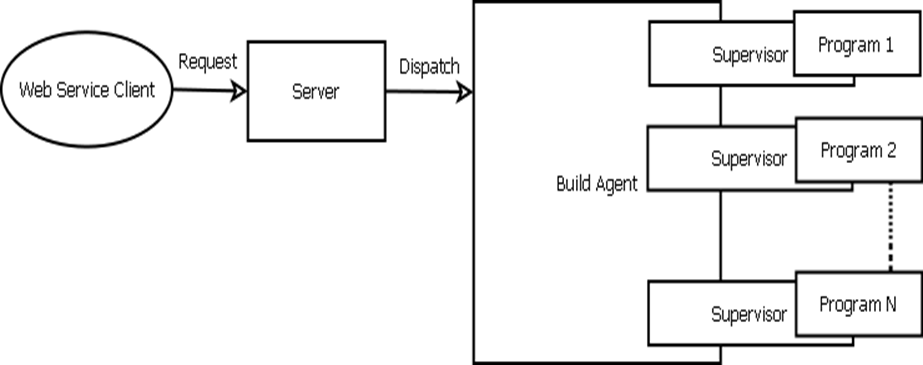
\includegraphics[scale=0.3]{pics/arch.png}
\caption{Arch model}
\end{center}
\label{fig2:arch}
\end{figure}


\section{Results}
\label{sec:results}
% vim: set tw=78 sts=2 sw=2 ts=8 aw et ai:

The project is functional.

As the date of this writing, it includes support for compiling/running code in the following languages:
\begin{enumerate}
\item{C}
\item{C++}
\item{Python}
\end{enumerate}

It also enables pasting and sharing code between peers, by generating a paste link.
When accessing the link, the code will be highlighted in the desired language, as can be seen from [fig3]

\begin{figure}
\begin{center}
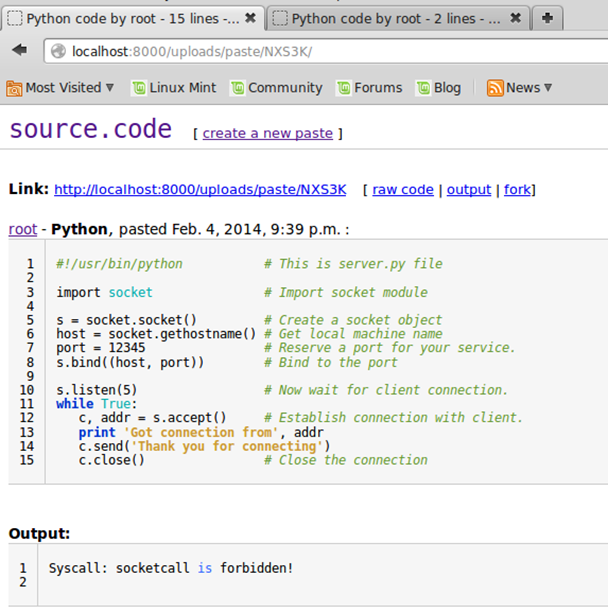
\includegraphics[scale=0.5]{pics/result.png}
\caption{Result}
\end{center}
\label{fig3:result}
\end{figure}


\section{Conclusion and Further Work}
\label{sec:conclusion}
% vim: set tw=78 sts=2 sw=2 ts=8 aw et ai:

There are three areas which have remained unattained, and with good reason, because of their complexity.
I plan on supporting these some time in the future.

\begin{enumerate}

\item{Different Architectures}

The current implementation is tied to the x86 architecture.
Current virtualization technologies are unfortunately very restrictive (It's hard to emulate PPC instruction set on a x86_64 bare metal).
This is why support for these kind of features in the industry is limited.
However, QEMU is a CPU simulator that is gaining more and more ground, and would be a good candidate for such a task.

\item{Different Language versions}

What is an user wants to compile a program using Python 2.6, or Python 3.0?. The same stands with C++98 vs C++11.
There is more than one standard for each language.
In order to provide support for this option, one would need a program that can change the runtime execution context.
Another option would be to have different VM's, each with its own run environment. 

\item{Kernel code}

Compiling and running kernel code is difficult, because once in the kernel one typically has control over the whole system.
Needless to say, we cannot simply compile kernel modules that users send, and insert them on our machine.
A possible solution to this problem would involve using User Mode Linux, which is Linux run inside a regular process, providing the regular encapsulation that processes have, and would allow us to hook up with the existing ptrace mechanism, that is already implemented.
\end{enumerate}


Writing SourceDotCode has been a challenging task. Although it still lacks some features, it's an useful tool to have around, when a compiler is missing.


% to be removed
\nocite{*}

\bibliographystyle{abbrv}
\bibliography{report}

\end{document}
